%! Author = borisdeletic
%! Date = 14/05/2023

% Preamble
\documentclass[11pt]{article}

% Document
\begin{document}
    \section{Nested Sampling}\label{sec:nested_sampling}
    Nested sampling is an algorithm which simultaneously computes
    the evidence and posterior~\cite{Skilling2006, Handley_polychord, NS_Review_2022}.
    For a set of parameters $\theta$, calculating the evidence through direct evaluation of the
    high-dimensional integral~\eqref{eq:evidence} becomes exponentially more expensive as the number of dimensions,
    $D$, is increased.

    We define the \emph{prior volume} as the fraction of prior contained within an iso-likelihood contour
    \begin{equation}\label{eq:prior_volume}
    X(\lambda) = \int_{\mathcal{L}(\theta)>\lambda} \pi(\theta) d\theta.
    \end{equation}
    Using a change of variable we write the evidence as a one-dimensional integral more feasible to calculate
    \begin{equation}\label{eq:evidence_ns}
    \mathcal{Z} = \int_0^1 {\mathcal{L}(X)} dX.
    \end{equation}

    Nested sampling introduces a population of $n_{\text{live}}$ \emph{live points} in the parameter space which are sorted
    by likelihood.
    These points are then iteratively updated to compress around the peaks of the posterior distribution.

    Initially, $n_{\text{live}}$ points are sampled from the prior $\pi(\theta)$.
    At each iteration $i$, the point with the lowest likelihood $\mathcal{L}_i$ is deleted and moved to the set
    of \emph{dead points}.
    A new live point is then generated from the prior, subject to the hard constraint that its likelihood is
    greater than $\mathcal{L}_i$.

    The prior volume on average will contract by a factor $n_{\text{live}}/(n_{\text{live}}+1)$ with each dead point, such that the
    expected prior volume at iteration $i$ will be
    \begin{equation}\label{eq:exp_prior_volume}
    \langle X_i \rangle = \left( \frac{n_{\text{live}}}{n_{\text{live}} + 1} \right)^i \approx e^{-i/n_{\text{live}}},
    \end{equation}
    thus compressing exponentially for large $n_{\text{live}}$.
    Each dead point has a likelihood $\mathcal{L}_i$, a set of parameters $\theta_i$, and a prior mass $X_i$, which can
    be used to estimate the evidence and posterior.

    \begin{figure}[t!]
        \center
        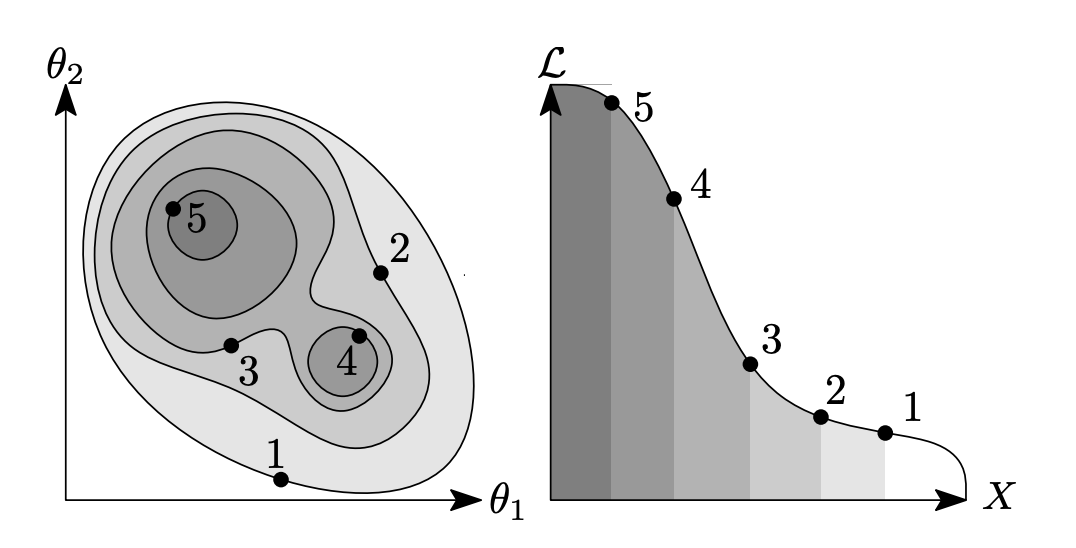
\includegraphics[width=\linewidth]{../figures/NestedSamplingPolychord}
        \caption{
            Nested sampling prior volume transformation. Left: Five sequentially higher iso-likelihood contours of a
            two-dimensional bimodal likelihood function $\mathcal{L}(\theta)$. Each contour encloses a smaller fraction
            of the prior volume $X$. Right: Likelihood $\mathcal{L}(X)$ as a function of enclosed volume $X$. The
            Bayesian evidence is the area under the curve.
            (Figure used from paper~\cite{Handley_polychord, Handley_2015}).
        }\label{fig:nested_sampling}
    \end{figure}

    Current state-of-the-art algorithms for nested sampling are able to calculate model evidences up to $D \sim 1,000$
    dimensions before the computational costs become overwhelming~\cite{Handley_2015, Feroz_2009, brewer2010diffusive}.

    \subsection{Evidence and Parameter Estimation}\label{subsec:evidence_param_estimation}
    We can use the dead points generated by the algorithm to computationally estimate the evidence.
    Approximating the integral~\eqref{eq:evidence_ns} using the trapezoid rule, we write
    \begin{equation}\label{eq:evidence_estimation}
    \mathcal{Z} = \sum_{i \in \text{dead}} w_i \mathcal{L}_i,
    \end{equation}
    where $w_i = (X_{i-1} - X_{i+1})/2$ is the weight factor estimating the change in prior volume per iteration.

    We can also use the dead points as samples from the posterior.
    Given that the $i$-th sample is assigned an importance weighting $w_i$, the posterior samples are
    \begin{equation}\label{eq:posterior_ns}
    p_i = \frac{w_i \mathcal{L}_i}{\mathcal{Z}} \propto w_i \mathcal{L}_i.
    \end{equation}

    We provide a further discussion of tuning nested sampling input parameters, and its effects on
    and evidence calculation and errors in~\cref{sec:ns_parameters}.

\end{document}